\begin{section}{XMSS and $XMSS^{MT}$}

    In this section, the XMSS/$XMSS^{MT}$ algorithms, as defined in the documents \cite{cooper2020recommendation} \cite{huelsing2018rfc} , will be explained using the fundamental structures presented in Section \ref{sec1}. Arhitecrure of the XMSS is given in the Figure \ref{fig:xmss}

\begin{figure}[h]
\centering
\begin{tikzpicture}[
    node distance=1.5cm,
    wots_pk/.style={rectangle, draw, fill=yellow!30, text width=1.5cm, align=center, minimum height=3cm},
    wots_sk/.style={rectangle, draw, fill=red!20, text width=1.5cm, align=center, minimum height=3cm},
    ltree_node/.style={circle, draw, fill=cyan!20},
    merkle_node/.style={circle, draw, fill=gray!20},
    leaf_node/.style={rectangle, draw, fill=green!20, minimum width=1cm},
    main_root/.style={merkle_node, fill=blue!30, label={[label distance=-2pt]90:\textbf{XMSS PK}}}
]

% WOTS+ Part
\node[wots_sk] (wots_sk) {WOTS+ Secret Key $sk_i$};
\node[wots_pk, right=of wots_sk] (wots_pk) {WOTS+ Public Key $pk_i$};
\draw[-Latex] (wots_sk) -- (wots_pk) node[midway, above] {$H^{w-1}$};

% L-Tree Part
\node[right=2cm of wots_pk] (ltree_label) {\textbf{L-Tree Compression}};
\node[ltree_node, below=0.5cm of ltree_label] (ltree_root) {$L_i$};
\node[ltree_node, below left=0.5cm and 0.2cm of ltree_root] (ltree1) {};
\node[ltree_node, below right=0.5cm and 0.2cm of ltree_root] (ltree2) {};
\draw (ltree1) -- (ltree_root) -- (ltree2);
\draw[-Latex, dashed] (wots_pk.east) .. controls +(0.5,0) and +(-0.5,0) .. (ltree_root.west);

% Merkle Tree Part
\node[right=2.5cm of ltree_root] (mt_label) {\textbf{Main Merkle Tree}};
\node[main_root, below=0.5cm of mt_label] (root) {};
\node[merkle_node, below left=0.7cm and 0.5cm of root] (n1) {};
\node[merkle_node, below right=0.7cm and 0.5cm of root] (n2) {};
\node[leaf_node, below left=0.7cm and 0.2cm of n1] (L0) {...};
\node[leaf_node, below right=0.7cm and 0.2cm of n1] (Li) {$L_i$};
\node[leaf_node, below left=0.7cm and 0.2cm of n2] (Lj) {...};
\node[leaf_node, below right=0.7cm and 0.2cm of n2] (LN) {...};
\draw (root) -- (n1) -- (L0);
\draw (n1) -- (Li);
\draw (root) -- (n2) -- (Lj);
\draw (n2) -- (LN);

% Connection from L-Tree to Merkle Tree
\draw[-Latex, thick, blue!60] (ltree_root.east) .. controls +(0.5,0) and +(-0.5,0) .. (Li.west);

% Signing part
\node[rectangle, draw, fill=orange!20, below=3cm of ltree_label] (msg) {Message Digest};
\draw[-Latex, dashed] (msg) -- (wots_sk.south) node[midway, right, text width=2cm] {Signed by};

\end{tikzpicture}
\caption{The architecture of XMSS. A WOTS+ key pair signs a message. Its public key is compressed via an L-Tree into a single leaf $L_i$. This leaf is part of a large Merkle tree, whose root serves as the overall XMSS public key.}
\label{fig:xmss}
\end{figure}


    \begin{subsection}{XMSS Key Generation}

        In Algorithm \ref{alg:XMSS_keygen}, a pseudo-code representation of the key generation process of the \textbf{XMSS} algorithm is provided. First, the \textbf{WOTS} private keys are generated. These keys can be created either completely at random or by passing a seed value through a key generation function. If all keys are generated randomly, they must be stored in memory for the signing process. However, since storing all the keys in memory is not realistic, this method is generally not used. Next, certain seed values are generated to be used throughout the algorithm, and the hash values of the WOTS private keys are taken to produce the WOTS public keys. In the pseudo-code, the value \texttt{idx} at the beginning of the \texttt{SK} section represents the state information.

        \begin{algorithm}
\caption{XMSS\_keyGen -- Generate an XMSS key pair}
\label{alg:XMSS_keygen}

\textbf{Input:} None \\
\textbf{Output:} XMSS private key \texttt{SK}, XMSS public key \texttt{PK}

\vspace{0.3cm}

\begin{tabular}{ll}
1: & \textit{// Example initialization for SK-specific contents} \\
2: & \texttt{idx} $\leftarrow 0$ \\
3: & \textbf{for} $i = 0$ \textbf{to} $2^h - 1$ \textbf{do} \\
4: & \quad \texttt{wots\_sk[i]} $\leftarrow$ \texttt{WOTS\_genSK()} \\
5: & \textbf{end for} \\
6: & Initialize \texttt{SK\_PRF} with a uniformly random $n$-byte string \\
7: & \texttt{setSK\_PRF(SK, SK\_PRF)} \\
8: & \textit{// Initialization for common contents} \\
9: & Initialize \texttt{SEED} with a uniformly random $n$-byte string \\
10: & \texttt{setSEED(SK, SEED)} \\
11: & \texttt{setWOTS\_SK(SK, wots\_sk)} \\
12: & \texttt{ADRS} $\leftarrow$ \texttt{toByte(0, 32)} \\
13: & \texttt{root} $\leftarrow$ \texttt{treeHash(SK, 0, h, ADRS)} \\
14: & \texttt{SK} $\leftarrow$ \texttt{idx $\parallel$ wots\_sk $\parallel$ SK\_PRF $\parallel$ root $\parallel$ SEED} \\
15: & \texttt{PK} $\leftarrow$ \texttt{OID $\parallel$ root $\parallel$ SEED} \\
16: & \textbf{return} \texttt{SK $\parallel$ PK}
\end{tabular}

\end{algorithm}

        
    \end{subsection}

    \begin{subsection}{XMSS Sign}

        In Algorithm \ref{alg:XMSS_sign}, the pseudo-code of the XMSS signing algorithm is presented. The \texttt{treeSig} function signs the message using WOTS and generates the authentication path required to reach the root of the tree. First, the state information is retrieved, then a random value is generated and concatenated with the message, after which a hash is computed from this combination. This hash value is then signed using the \texttt{treeSig} algorithm. The final signature consists of the concatenation of the state information, the random value, and the \texttt{treeSig} signature, respectively.


        \begin{algorithm}
\caption{XMSS\_sign – Generate an XMSS signature and update the XMSS private key}
\label{alg:XMSS_sign}

\textbf{Input:} Message $M$, XMSS private key $SK$ \\
\textbf{Output:} Updated $SK$, XMSS signature $Sig$

\vspace{0.3cm}

\begin{tabular}{ll}
1: & \texttt{idx\_sig} $\leftarrow$ \texttt{getIdx(SK)} \\
2: & \texttt{setIdx(SK, idx\_sig + 1)} \\
3: & \texttt{ADRS} $\leftarrow$ \texttt{toByte(0, 32)} \\
4: & \texttt{r} $\leftarrow$ \texttt{PRF(getSK\_PRF(SK), toByte(idx\_sig, 32))} \\
5: & \texttt{M'} $\leftarrow$ \texttt{H\_msg(r $\parallel$ getRoot(SK) $\parallel$ toByte(idx\_sig, n), M)} \\
6: & \texttt{Sig} $\leftarrow$ \texttt{idx\_sig $\parallel$ r $\parallel$ treeSig(M', SK, idx\_sig, ADRS)} \\
7: & \textbf{return} \texttt{SK $\parallel$ Sig}
\end{tabular}

\end{algorithm}

        
\end{subsection}

\begin{subsection}{XMSS Verify}

In Algorithm \ref{alg:xmss_rootfromSign} and \ref{alg:xmss_verify}, the pseudo-code of the XMSS signature verification is presented. First, the WOTS public key is derived from the message. Then, these WOTS public keys are passed through the \texttt{L-tree} to obtain the leaves of the Merkle tree. From the leaves of the Merkle tree, the root is reached to obtain the XMSS public key and perform verification. If the derived public key matches the expected value, the signature is considered valid. The authentication path contained in the signature is used to climb to the root in both the \texttt{L-tree} and the Merkle tree.

\begin{algorithm}
\caption{XMSS\_rootFromSig: Compute a root node from a tree signature}
\label{alg:xmss_rootfromSign}

\textbf{Input:} \\
\quad index \texttt{idx\_sig} \\
\quad WOTS+ signature \texttt{sig\_ots} \\
\quad authentication path \texttt{auth} \\
\quad $n$-byte message $M'$ \\
\quad seed \texttt{SEED} \\
\quad address \texttt{ADRS} \\[0.2cm]
\textbf{Output:} $n$-byte root value \texttt{node[0]}

\vspace{0.3cm}

\begin{tabular}{ll}
1: & \texttt{ADRS.setType(0)} \hfill \textit{// Type = OTS hash address} \\
2: & \texttt{ADRS.setOTSAddress(idx\_sig)} \\
3: & \texttt{pk\_ots} $\leftarrow$ \texttt{WOTS\_pkFromSig(sig\_ots, M', SEED, ADRS)} \\
4: & \texttt{ADRS.setType(1)} \hfill \textit{// Type = L-tree address} \\
5: & \texttt{ADRS.setLTreeAddress(idx\_sig)} \\
6: & Initialize \texttt{node[0]} and \texttt{node[1]} as $n$-byte arrays \\
7: & \texttt{node[0]} $\leftarrow$ \texttt{ltree(pk\_ots, SEED, ADRS)} \\
8: & \texttt{ADRS.setType(2)} \hfill \textit{// Type = hash tree address} \\
9: & \texttt{ADRS.setTreeIndex(idx\_sig)} \\
10: & \textbf{for} $k = 0$ \textbf{to} $h-1$ \textbf{do} \\
11: & \quad \texttt{ADRS.setTreeHeight(k)} \\
12: & \quad \textbf{if} $\left\lfloor \texttt{idx\_sig} / 2^k \right\rfloor \bmod 2 = 0$ \textbf{then} \\
13: & \qquad \texttt{ADRS.setTreeIndex(ADRS.getTreeIndex() / 2)} \\
14: & \qquad \texttt{node[1]} $\leftarrow$ \texttt{RAND\_HASH(node[0], auth[k], SEED, ADRS)} \\
15: & \quad \textbf{else} \\
16: & \qquad \texttt{ADRS.setTreeIndex((ADRS.getTreeIndex() - 1) / 2)} \\
17: & \qquad \texttt{node[1]} $\leftarrow$ \texttt{RAND\_HASH(auth[k], node[0], SEED, ADRS)} \\
18: & \quad \textbf{end if} \\
19: & \quad \texttt{node[0]} $\leftarrow$ \texttt{node[1]} \hfill \textit{// Update current node} \\
20: & \textbf{end for} \\
21: & \textbf{return} \texttt{node[0]}
\end{tabular}

\end{algorithm}


        \begin{algorithm}
        \caption{XMSS\_verify -- Verify an XMSS signature using the corresponding XMSS public key and a message}
        \label{alg:xmss_verify}
        \textbf{Input:} XMSS signature \texttt{Sig}, message \texttt{M}, XMSS public key \texttt{PK} \\
        \textbf{Output:} Boolean
        
        \vspace{0.2cm}
        
        \begin{tabular}{ll}
        1: & \texttt{ADRS} $\leftarrow$ \texttt{toByte(0, 32)} \\
        2: & \texttt{M'} $\leftarrow$ \texttt{H\_msg(r || getRoot(PK) || toByte(idx\_sig, n), M)} \\
        3: & \texttt{node} $\leftarrow$ \texttt{XMSS\_rootFromSig(idx\_sig, sig\_ots, auth, M', getSEED(PK), ADRS)} \\
        4: & \textbf{if} \texttt{node == getRoot(PK)} \textbf{then} \\
        5: & \hspace{0.5cm} \textbf{return} \texttt{true} \\
        6: & \textbf{else} \\
        7: & \hspace{0.5cm} \textbf{return} \texttt{false} \\
        8: & \textbf{end if}
        \end{tabular}
        
        \end{algorithm}
        
    \end{subsection}

    \begin{subsection}{$XMSS^{MT}$}
        $XMSS^{MT}$ is the multi-tree version of the XMSS algorithm. While the XMSS algorithm consists of a single large tree, the multi-tree structure comprises many smaller trees, each signing the public key of the next. The advantage of this approach is that signing is faster because it eliminates the need to generate the entire large tree during the signature verification process. In a multi-tree structure, the signature is formed by the combination of the signatures and authentication paths of each layer. Figure \ref{fig:MTsig} shows the multi-tree signature structure. Figure \ref{fig:MTstruc} illustrates the overall structure of the multi-tree.

        


        \begin{figure}
        \centering
        \begin{subfigure}{0.5\textwidth}
          \centering
          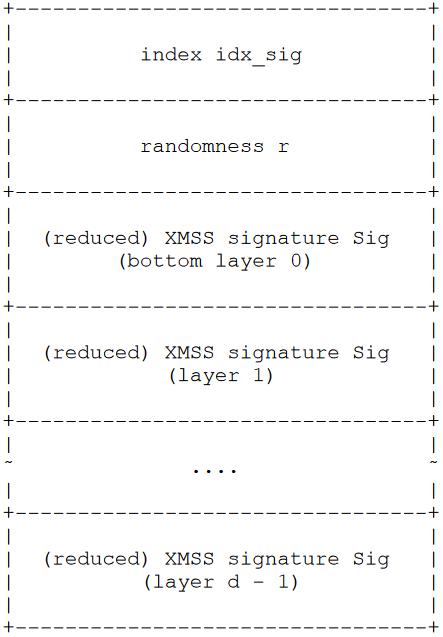
\includegraphics[width=\linewidth]{fig/MTsignature.png}
          \caption{Multi-tree signature}
          \label{fig:MTsig}
          
        \end{subfigure}%
        \begin{subfigure}{0.5\textwidth}
          \centering
          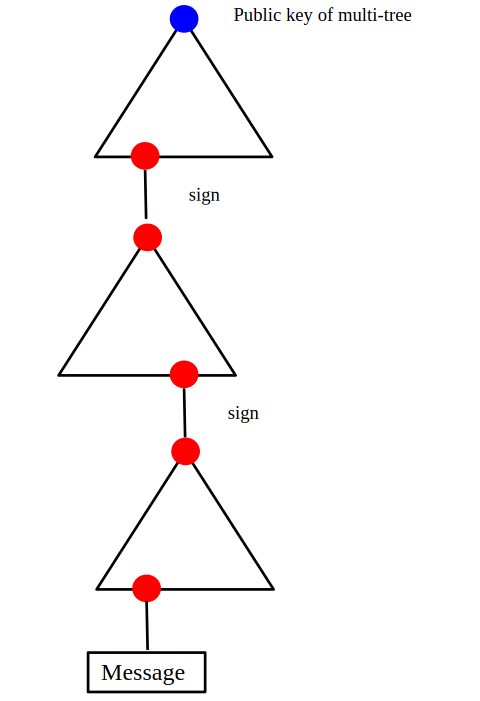
\includegraphics[width=\linewidth]{fig/multi-tree.png}
          \caption{Multi-tree general structure}
          \label{fig:MTstruc}
          
        \end{subfigure}
        \caption{XMSS multi-tree}
        \label{fig:LAT}
        \end{figure}


        
    \end{subsection}

    
    
\end{section}